%
%
% Kapitel Datensimulation
%
%


\chapter{Datensimulation und -rekonstruktion}

\section{Monte-Carlo-Simulation}

Ein Vergleich der Ergebnisse aus von CMS gemessenen Daten mit Monte-Carlo-Simulationen ist eine gute Methode, die Messergebnisse mit Vorhersagen des Standardmodells, aber auch mit Modellen, die davon abweichen, zu vergleichen. Das Ziel der Datensimulation ist es, mithilfe von Zufallsgeneratoren und physikalischer Modelle Pseudodaten zu erzeugen. Diese Pseudodaten liegen dann im selben Datenformat vor, in dem auch die echten Daten zur Verf�gung stehen. Somit k�nnen dieselben Analysen sowohl auf gemessene als auch auf simulierte Daten angewendet werden. In diesem Kapitel wird erl�utert, wie die in dieser Analyse untersuchten simulierten Daten produziert werden.

\subsection{Produktionskette}

Die Simulation der Daten erfolgt in mehreren, aufeinander aufbauenden Schritten. Diese sind im Einzelnen:

\begin{enumerate}
	\item Numerische Integration des Matrixelementes (ME) des harten Prozesses und Berechnung des Wirkungsquerschnittes daraus.
	\item Ereignisgeneration: Partonen und Leptonen im Anfangs- und Endzustand der harten Interaktion werden, unter Beachtung der erwarteten Wahrscheinlichkeiten, zuf�llig erzeugt.
	\item Modellierung von Teilchenschauern: Die Abstrahlung von Gluonen und Photonen aus den Teilchen im Anfangs- und Endzustand wird simuliert.
	\item Hadronisierung: Gruppierung von Quarks zu farbneutralen Hadronen.
	\item Hadronischer Zerfall: Der Zerfall von kurzlebigen Teilchen wird reproduziert.
	\item Underlying Event (UE): Hinzuf�gen von Teilchen im Endzustand, die von Protonr�ckst�nden aus dem harten Prozess entstehen.
	\item Pileup: Eine zuf�llige Anzahl von zus�tzlichen, weichen Proton-Proton-Kollisionen wird erzeugt und dem Ereignis hinzugef�gt.
	\item Detektorsimulation: Die Wechselwirkung der in Schritt 2 bis 7 produzierten Teilchen mit dem Detektormaterial und die Detektorantwort werden simuliert.
\end{enumerate}

\subsection{Simulation von $t\overline{t}+\gamma$ Ereignissen}

F�r die Simulation des $t\overline{t}+\gamma$-Signals wurde WHIZARD, ein Leading-Order-Monte-Carlo-Generator, benutzt. Ein Schaubild mit verschiedenen simulierbaren Endzust�nden der Monte-Carlo-Generation ist in Abb.\ref{fig:whizard} gezeigt, auf diese soll hier kurz eingegangen werden:

\begin{description}
  \item[2 $\rightarrow$ 3:] Hier werden nur quantenmechanische Interferenzen aus Photonabstrahlungen von Teilchen im Anfangszustand betrachtet. Der Vorteil dieses Modells ist die geringe CPU-Last, die bei der Berechnung der ME anf�llt, es zeigt sich aber, da� die Physik hier nicht korrekt beschrieben wird. \cite{Tholen:Master}
	\item[2 $\rightarrow$ 5:] In diesem Modell ist der Zerfall der Top-Quarks ber�cksichtigt, hier tr�gt nun auch die Photonabstrahlung der W-Bosonen und der b-Quarks zum Signal bei. Es stellt einen guten Kompromiss dar zwischen CPU-Auslastung und korrekter Beschreibung der Natur und wird in dieser Analyse benutzt.
	\item[2 $\rightarrow$ 7:] Hier werden alle Photonabstrahlungen des harten Prozesses ber�cksichtigt und die realen Prozesse am besten beschrieben, diese Strategie ist jedoch �beraus CPU-intensiv und wird in dieser Analyse nicht weiter untersucht.
\end{description}

\begin{figure}%
\centering
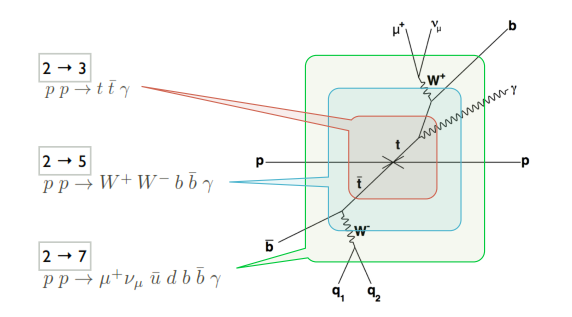
\includegraphics[width=0.7\columnwidth]{bilder/whizard}%
\caption{Strategien der Ereignisgeneration mit WHIZARD. \cite{Tholen:Master}}%
\label{fig:whizard}%
\end{figure}

WHIZARD benutzt die Partondichteverteilung CTEQ6L1 und eine variable Renormalisierungs- und Faktorisierungsskala. Diese Skalen werden f�r jedes Ereignis auf einen Wert von 172,5\,GeV ($m_t$) plus der Transversalenergie des erzeugten Photons festgelegt. Die Teilchenschauer der Anfangs- und Endzust�nde sowie die Hadronisierung werden von PYTHIA6, TAUOLA und PHOTOS simuliert, dabei wird dieselbe Konfiguration wie f�r das Top-Paar-Sample benutzt. \
An die Teilchen im Endzustand werden bestimmte Anforderungen gestellt, sogenannte "`Produktionsschnitte"'. So wird eine minimale transversale Energie gefordert, um Infrarotdivergenz entgegenzuwirken und eine Minimaldistanz im $\eta-\Phi$-Raum gegen kollineare Divergenz. In dieser Analyse wird eine minimale Transversalenergie des Photons und beider b-Quarks von 10\,GeV und ein $\Delta R > 0,1$ zwischen dem Photon und jedem anderen Teilchen im Endzustand gefordert. Die Messung wird davon nicht beeinflusst, da die Schnitte in der Ereignisselektion noch h�rter sind.

\subsection{Simulation des Top-Paar-Prozesses und der betrachteten Untergr�nde}

Die meisten Monte-Carlo-Simulationen neben den $t\overline{t}+\gamma$-Ereignissen wurden mit MADGRAPH generiert, hier wurde die Partondichtefunktion CTEQ6L1 benutzt. Single-Top-Ereignisse wurden mit POWHEG simuliert, der Zerfall des $\tau$-Leptons mittels TAUOLA. Die Hadronisierung sowie die Teilchenschauer wurden mit PYTHIA (hadronische Wechselwirkung) sowie PHOTOS (elektromagnetische Wechselwirkung) modelliert.\
Der Phasenraum der Ereignisse der WHIZARD $t\overline{t}+\gamma$-Simulation ist im MADGRAPH $t\overline{t}$-Sample schon abgedeckt. Deswegen werden Ereignisse aus dem $t\overline{t}$-Sample, welche die Produktionsschnitte in WHIZARD auf Partonebene erf�llen, nicht ber�cksichtigt, um diese �berschneidung zu entfernen.

\subsection{Detektorsimulation}

Der Durchgang der von den Monte-Carlo-Generatoren erzeugten Teilchen durch die einzelnen Detektorkomponenten sowie die dadurch ausgel�sten Signale werden mit dem Programm GEANT4 modelliert. GEANT4 simuliert anhand der Detektorgeometrie und des Magnetfeldes das Verhalten der einzelnen Teilchen im Detektor. Dabei werden alle elektromagnetischen und hadronischen Wechselwirkungen mit dem Detektormaterial ber�cksichtigt, wie z.B. Schauer in den Kalorimetern. Trifft ein Teilchen aktives Detektormaterial, erzeugt die Simulation das elektrische Signal, welches auch bei einer Messung entstehen w�rde und simuliert die elektronische Auslese der Signale, die Digitalisierung, in den unterschiedlichen Detektorkomponenten. Die Ausgabe der Digitalisierung wird gespeichert und sp�ter in der Rekonstruktion der einzelnen Teilchen verwendet. Diese Rekonstruktion erfolgt mit den gleichen Algorithmen wie die Rekonstruktion experimenteller Daten. Neben der vollst�ndigen Simulation des Detektors ("`FullSim"'), die viel Rechenzeit und -aufwand ben�tigt, wurden auch vereinfachte Modelle zur Detektorsimulation entwickelt ("`FastSim"'). Dadurch werden die Dauer der Simulation und der ben�tigte Speicherplatz erheblich reduziert. Die Daten in dieser Analyse werden mittels FullSim prozessiert.

\section{Ereignisrekonstruktion}

Die Ereignisrekonstruktion erstellt aus den Messwerten der verschiedenen Subdetektoren Kandidaten f�r physikalische Objekte wie z.B. Myonen, Elektronen, Photen oder Jets und verwendet dazu die digitalisierten Ausgangssignale des Detektors. Abbildung\ref{fig:reco} zeigt einen Ausschnitt des CMS-Detektors und die unterschiedlichen Signaturen, die beim Teilchendurchgang durch den Detektor erzeugt werden. Als einzige detektierbare Teilchen durchqueren Myonen den gesamten Detektor und hinterlassen Spuren in allen Subdetektoren. Bei hohen Energien dominiert f�r Elektronen der Energieverlust durch Bremsstrahlung. Diese hinterlassen daher nur einen Eintrag im Spurdetektor und werden im elektromagnetischen Kalorimeter gestoppt. Photonen sind elektrisch neutral und hinterlassen somit nur Eintr�ge im elektromagnetischen Kalorimeter. Stark wechselwirkende Teilchen sind in den meisten F�llen geladen und hinterlassen somit auch eine Spur im Spurdetektor, weiterhin deponieren sie Energie im elektromagnetischen und im hadroonischen Kalorimeter. \
Die Rekonstruktion untersucht diese Signaturen, um R�ckschl�sse auf die erzeugten Teilchen zu ziehen. In der CMS Kollaboration werden sogenannte "`Particle Object Groups"' (POG) gebildet, die sich auf die Rekonstruktion einzelner Teilchenarten spezialisieren und die Objekte definieren, mit denen in Physik-Analysen gearbeitet wird. Im folgenden wird ein kurzer �berblick gegeben, wie verschiedene Objekte zu Leptonen oder Jets rekonstruiert werden.

\begin{figure}%
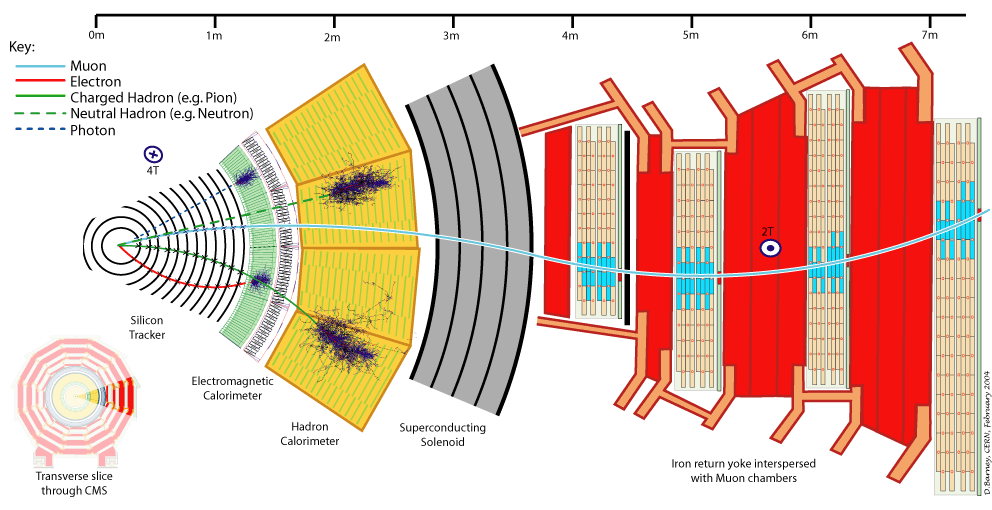
\includegraphics[width=\columnwidth]{bilder/reco}%
\caption{Ein Ausschnitt des CMS Detektors mit Signaturen verschiedener Teilchen \cite{CMS:Slice}}%
\label{fig:reco}%
\end{figure}

\subsection{Myonen}

